\chapter{Propuesta de trabajo}
\label{cha:Propuesta de trabajo}

\begin{FraseCelebre}
  \begin{Frase}
    Texto.
  \end{Frase}
  \begin{Fuente}
    Autor texto
  \end{Fuente}
\end{FraseCelebre}

\noindent
Este trabajo se encuentra realizado dentro del del proyecto \ac{T4AC} desarrollado en el grupo RobeSafe de la Universidad de Alcalá. El grupo de investigación RobeSafe dirigido por Luis Miguel Bergasa, trata de conseguir sistemas de conducción más seguros mediante la creación y el diseño de un vehículo autónomo. Tras la realización del \ac{TFG} titulado 'Algoritmos de detección de objetos 3D basados en LiDAR: comparación entre técnicas PCL clásicas y Deep Learning' \cite{tfg_javi} dentro de este grupo, se finalizó con la realización de un sencillo sistema de fusión sensorial entre cámara y \ac{LiDAR}. Dicho sistema se encontraba basado en una late-fusion, ya que en dicho \ac{TFG} se estudia principalmente las técnicas de detección utilizando únicamente \ac{LiDAR}, por lo que la fusión se realizó junto con un compañero del grupo RobeSafe \cite{tfg_miguel}.

Gracias al trabajo realizado previamente se comprenden las limitaciones de los diferentes sensores utilizados en los vehículos autónomos para la percepción del entorno. Por ello se plantea el diseño y creación de un sistema de detección 3D basado en una middle-fusion entre cámara y \ac{LiDAR}. Antes de la decisión del tipo de sistema se definen las principales características del sistema a implementar: el sistema tiene que ser utilizable en tiempo real y debe de producir menos falsos positivos que un sistema de detección 3D en tiempo real como puede ser PointPillars \cite{PointPillars} o SECOND \cite{SECOND}, debido a que utiliza de forma adicional la información proporcionada por la cámara.

Tras estudiar múltiples papers del estado del arte en fusión sensorial como los presentados en el Capítulo \ref{cha:Estado del arte en técnicas de fusión sensorial}, se comienza a diseñar la arquitectura del modelo a construir. Primero se plantea el uso de un sistema de detección 2D sobre la cámara como base del modelo a construir, debido a la gran precisión de los modelos de detección 2D basados en cámara, además de la gran velocidad de ejecución de dichos modelos, en contraposición a modelos como PointPainting \cite{PointPainting} que se basan en modelos más lentos de segmentación semántica.

La tarea más compleja en los modelos de detección 3D basados en cámara, es la obtención de la distancia a los objetos que quieren ser detectados. Para solucionar esta tarea, se plantea el uso de técnicas analíticas clásicas como las vistas en el desarrollo del Máster Universitario en Analítica de Negocio y Big Data, ya que pueden permitir la obtención de una aproximación de la distancia al objeto sin necesidad de redes neuronales, al contrario de como ocurre con el modelo Frustum PointNets \cite{Frustum_PointNets}. Esta aproximación requeriría de un ajuste en varias fases, tal como en el modelo PointRCNN \cite{PointRCNN}, donde las detecciones se producen en múltiples pasos para obtener mejores detecciones finales. Para dicha aproximación por tanto, se estudiarán las características de la cámara, las detecciones 2D obtenidas y la nube de puntos, para obtener un aproximación de la distancia a cada uno de los objetos a detectar del entorno.

Obtenidas las detecciones 2D de los objetos del entorno junto con una distancia aproximada a cada uno de los objetos, se estudiarán las transformaciones entre cámara y \ac{LiDAR}, para la generación de troncos de pirámide con la nube de puntos que incluya el objeto a detectar. Dicho proceso puede simplificar la etapa de detección 3D final, ya que permite detectar un solo objeto por región de interés. Por lo que cuanto más pequeña sea la región de interés, más fácil será para el modelo obtener las detecciones finales y menos puntos será necesario que analice, por lo que se reduciría el tiempo de computo.

\begin{figure}[H]
    \centering
    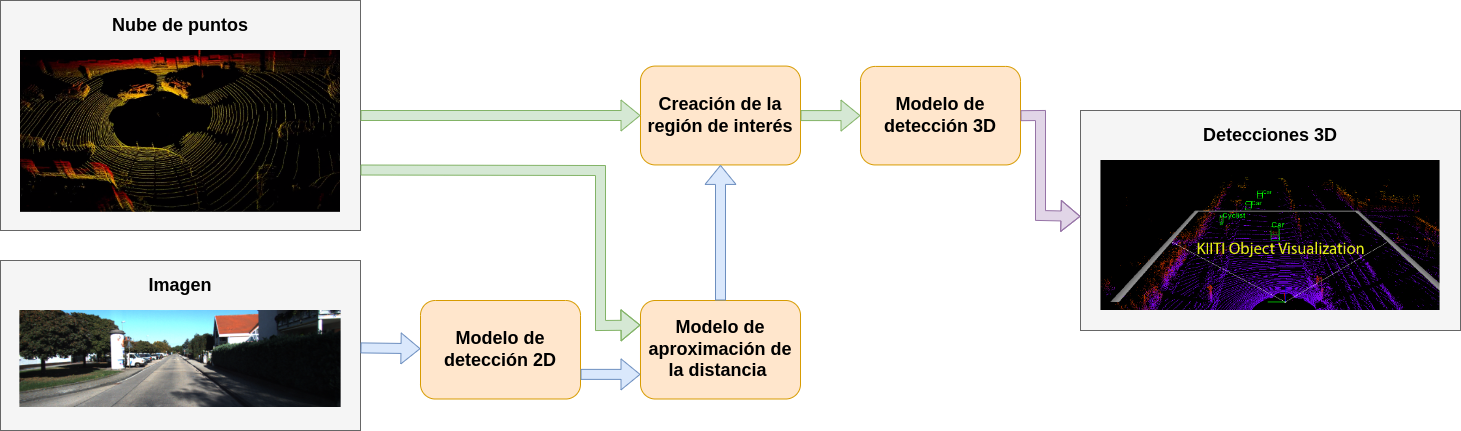
\includegraphics[width=1\textwidth]{Book/figures/3_propuesta/propuesta.drawio.png}
    \caption{Arquitectura propuesta.}
    \label{fig:Arquitectura propuesta.}
\end{figure}

Como fase final se plantea el uso de un modelo basado en Deep Learning sobre cada una de las regiones de interés en las que se encuentran los objetos. El modelo que se decida utilizar deberá de aprovechar el echo de trabajar con una región de interés de menor tamaño para acelerar el proceso de obtención de las detecciones 3D, ya que la velocidad tiene que ser uno de los factores más importantes en el proceso de creación de esta arquitectura. De forma adicional se podría aplicar un proceso de inferencia de las bounding boxes 3D por cada uno de los objetos mediante una ejecución por batches (agrupando los datos para su entrada en el modelo), ya que conseguiría obtener las detecciones finales utilizando el modelo planteado de forma paralela en GPU, y no de forma secuencial como se podría hacer de forma más sencilla.

El diseño de esta arquitectura pretende ayudar a la implantación de un sistema de detección 3D en el vehículo \ac{T4AC} del grupo RobeSafe, ya que al utilizar sistemas de procesamiento embebidos como: NVIDIA Jetson y Raspberry Pi; no se tiene mucha potencia de computo, y este tipo de arquitectura puede ayudar en la implementación del sistema de detección en tiempo real en dicho vehículo. Definida la aplicabilidad de esta arquitectura a crear (aunque no se pretenda implementar en el vehículo real), se decanta por el uso del dataset de KITTI para la creación y evaluación de todo este sistema al ser basarse en un sistema de sensores muy similar del vehículo \ac{T4AC}, consistente de una cámara estéreo frontal y un \ac{LiDAR} con visión en 360º.

En resumen, se estudiará el dataset KITTI para la creación de un sistema de detección 3D entre cámara y \ac{LiDAR}. Dicho sistema consistirá en 4 etapas: detección 2D, aproximación de la distancia, extracción de la región de interés y detección 3D final; este flujo de trabajo se muestra en la Figura \ref{fig:Arquitectura propuesta.} para comprender de forma más sencilla que se quiere realizar. Por último, la arquitectura creada será evaluada sobre KITTI para compararse con otros modelos y comprender si esta aproximación tiene sentido en términos de precisión y tiempo de inferencia comparando con el estado del arte.
